\section{Evaluation: Recasting Type Errors as Runtime Errors}
\label{sec:eval-witness}
%
The immediate question is ``What fraction of type errors admit
witnesses?''
%
To answer this question we implemented a prototype of our search
procedure for the pure subset of \ocaml, \ie \lang extended with
algebraic datatypes and records. 
%
In our implementation we instantiated \gensym with a simple random
generation of values, which we will show is more than sufficient for the
majority of type errors.
%
We evaluated our implementation of two sets of known-bad programs, \ie
programs that were rejected by the \ocaml compiler because of a type
error.
%
The first dataset comes from the Spring 2014 undergraduate Programming
Languages course at UC San Diego (IRB \#140608). 
%
We recorded each interaction with the \ocaml top-level system over the
course of the first three assignments, from which we extracted XXXX
distinct, ill-typed \ocaml programs.
%
The second dataset -- widely used in the literature -- comes from a
similar course at the University of
Washington~\cite{lerner_seminal:_2006}, from which we extracted 284
ill-typed programs.

We ran our search algorithm on each program with the entry point set to
the function that \ocaml had identified as containing a type error. 
%
Due to the possibility of non-termination we set a limit on the number
of reductions to perform, increasing in 500-step increments from 500
steps to 3,000 steps total.
%
We also added a na\"ive check for infinite recursion; at each recursive
function call we check whether the new arguments are identical to the
current arguments.
%
If so, the function cannot possibly terminate and we report an error.
%
While not a \emph{type error}, infinite recursion is still a clear bug
in the program, and thus valuable feedback for the user.

\begin{figure}[t]
\centering
\begin{minipage}{\linewidth}
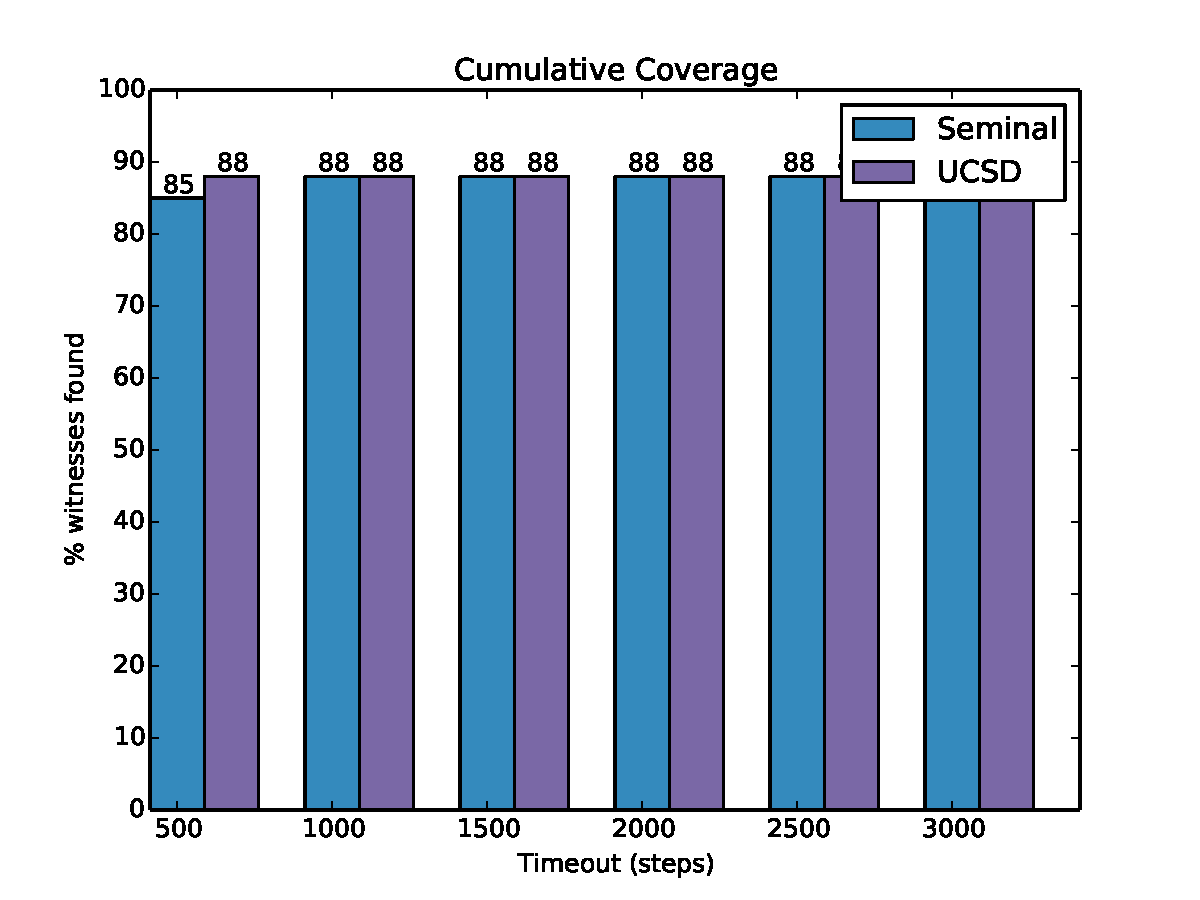
\includegraphics[width=\linewidth]{coverage.pdf}
\end{minipage}
\begin{minipage}{\linewidth}
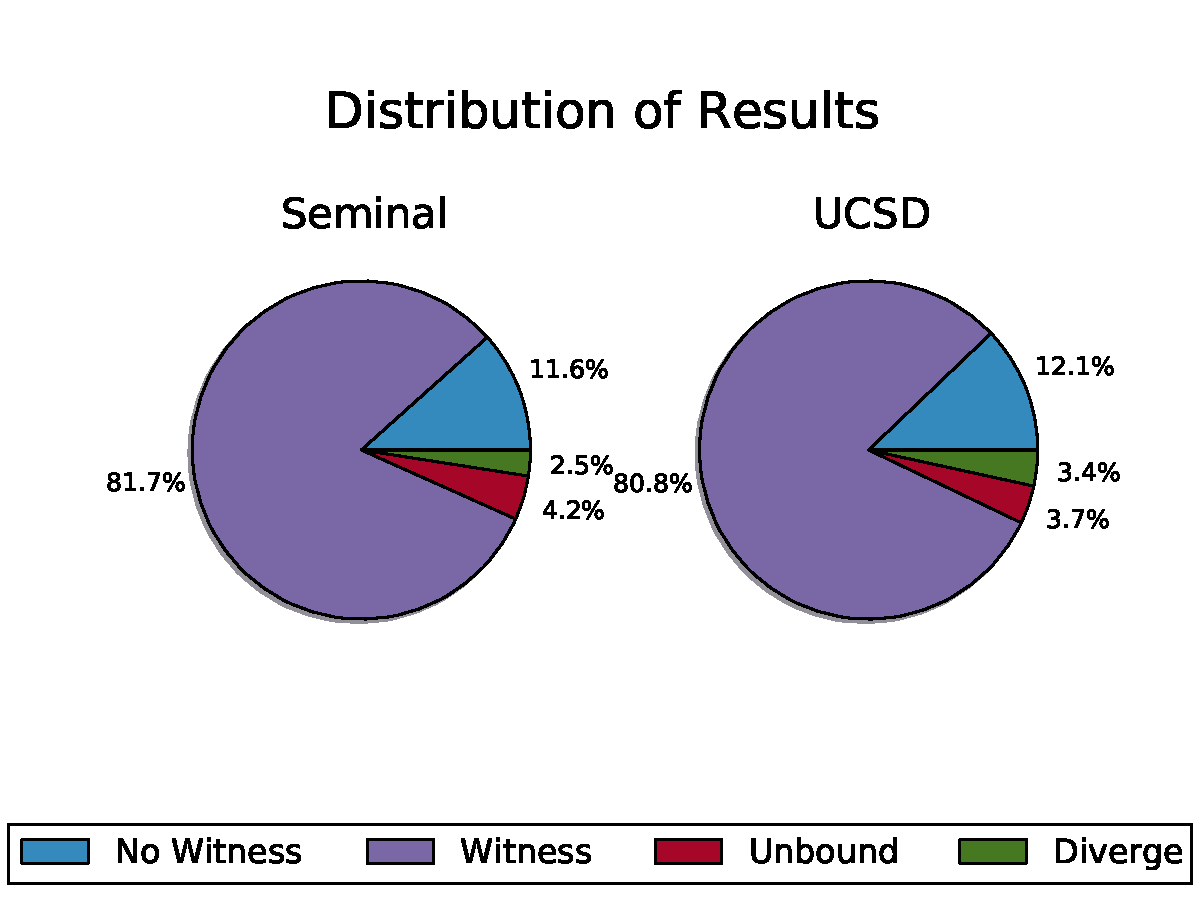
\includegraphics[width=\linewidth]{distrib.pdf}
\end{minipage}
\vspace{-8ex}
\caption{Experimental results. Our random search successfully finds
  witnesses for over 85\% of the programs at the lowest timeout and
  improves slightly to 88\% at the next level. In both datasets we
  detect actual type errors about 82\% of the time, unbound variables or
  constructors 3-4\% of the time, and diverging loops 2-3\% of the
  time. For the remaining 11-12\% of the programs we are unable to
  provide any useful feedback. \ES{TODO: the timeout number for ucsd is
    a bit misleading due to a mistake in the benchmarking code. re-running to fix..}
}
\label{fig:results-witness}
\end{figure}

\paragraph{Results}
\label{sec:results-witness}
The results of our experiments are summarized in
Figure~\ref{fig:results-witness}.
%
In both datasets our tool was able to find a witness for at least XX\%
of the programs.
%
Interestingly, while the vast majority of witnesses corresponded to a
type-error, as expected, X\% triggered an unbound variable error and X\%
triggered an infinite recursion error.
%
XX programs were deemed safe and XX timed out even at 3,000 steps, \ie
we could not provide any useful feedback for XX\% of the total programs.
%
While a more advanced search procedure, \eg dynamic-symbolic execution,
could likely trigger more of the type errors, our experiments show that
type errors are coarse enough (or that novice programs are \emph{simple}
enough) that these techniques are not necessary.



% \begin{itemize}
% \item benchmarks: our data + seminal data
% \item both cases: \textbf{random} search sufficient to trigger runtime crash in 80\% of programs
% \item how many of the ``safe'' programs are actually safe??
% \end{itemize}
